\documentclass[12pt,a4paper]{article}
\usepackage[top=1.5cm, bottom=1.5cm, left=2.0cm, right=1.5cm] {geometry}
\usepackage{amsmath,amssymb,fontawesome}
\usepackage{tkz-euclide}
\usepackage{setspace}
\usepackage{lastpage}

\usepackage{tikz,tkz-tab}
%\usepackage[solcolor]{ex_test}
\usepackage[dethi]{ex_test} % Chỉ hiển thị đề thi
%\usepackage[loigiai]{ex_test} % Hiển thị lời giải
%\usepackage[color]{ex_test} % Khoanh các đáp án
\usetikzlibrary{shapes.geometric,arrows,calc,intersections,angles,quotes,patterns,snakes,positioning}
\everymath{\displaystyle}

\def\colorEX{\color{purple}}
%\def\colorEX{}%Không tô màu đáp án đúng trong tùy chọn loigiai
\renewtheorem{ex}{\color{violet}Câu}
\renewcommand{\FalseEX}{\stepcounter{dapan}{{\bf \textcolor{blue}{\Alph{dapan}.}}}}
\renewcommand{\TrueEX}{\stepcounter{dapan}{{\bf \textcolor{blue}{\Alph{dapan}.}}}}

%---------- Khai báo viết tắt, in đáp án
\newcommand{\hoac}[1]{ %hệ hoặc
    \left[\begin{aligned}#1\end{aligned}\right.}
\newcommand{\heva}[1]{ %hệ và
    \left\{\begin{aligned}#1\end{aligned}\right.}

%Tiêu đề
\newcommand{\tenso}{}
\newcommand{\tentruong}{LỚP TOÁN 12}
\newcommand{\tenkythi}{ĐỀ ÔN TẬP}
\newcommand{\tenmonthi}{Môn học: }
\newcommand{\thoigian}{}
\newcommand{\tieude}[1]{
    \noindent
     \begin{minipage}[b]{6cm}
    \centerline{\textbf{\fontsize{11}{0}\selectfont \tenso}}
    \centerline{\fontsize{11}{0}\selectfont \tentruong}  
  \end{minipage}\hspace{1cm}
  \begin{minipage}[b]{11cm}
    \centerline{\textbf{\fontsize{11}{0}\selectfont \tenkythi}}
    \centerline{\textbf{\fontsize{11}{0}\selectfont \tenmonthi}}
    \centerline{\textit{\fontsize{11}{0}\selectfont Thời \underline{gian làm bài: \thoigian  } phút }}
  \end{minipage}
  \vspace*{3mm}
  \noindent
  \begin{minipage}[t]{12cm}
    \textbf{Họ, tên thí sinh:}\dotfill\\
    \textbf{Số báo danh:}\dotfill
  \end{minipage}\hfill
  \begin{minipage}[b]{3cm}
    \setlength\fboxrule{1pt}
    \setlength\fboxsep{3pt}
    \vspace*{3mm}\fbox{\bf Mã đề thi #1}
  \end{minipage}\\
}

\newcommand{\chantrang}[2]{\rfoot{Trang \thepage $-$ Mã đề #2}}
\pagestyle{fancy}
\fancyhf{}
\renewcommand{\headrulewidth}{0pt} 
\renewcommand{\footrulewidth}{0pt}

\begin{document}
%Thiết lập giãn dọng 1.5cm 
%\setlength{\lineskip}{1.5em}



%Nội dung trắc nghiệm bắt đầu ở đây


\tieude{001}
\chantrang{\pageref{LastPage}}{001}
\setcounter{page}{1}
{\bf PHẦN II. Câu trắc nghiệm đúng sai.}
\setcounter{ex}{0}
\Opensolutionfile{ans}[ans/ans001-2]
\begin{ex}
 Đường gấp khúc ${ABC}$ trong hình bên là đồ thị của hàm số $y=f(x)$ trên đoạn ${[-3;0]}$. Xét tính đúng-sai của các khẳng định sau. 
\begin{center}
 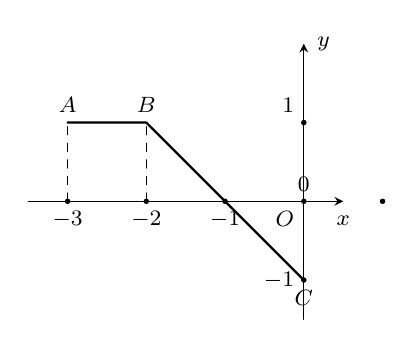
\begin{tikzpicture}[scale=1,>=stealth, font=\footnotesize, line join=round, line cap=round]
            \tikzset{label style/.style={font=\footnotesize}}
            \def \xmin{-3.5}\def \xmax{0.5}\def \ymin{-1.5}\def \ymax{2}
            \draw[->] (\xmin,0)--(\xmax,0) node[shift=(-90:0.25)] {$x$};
            \draw[->] (0,\ymin)--(0,\ymax) node[shift=(0:0.25)] {$y$};
            \foreach \x in {-3,-2,-1,}
            \fill[black] (\x,0) node[below]{$\x$}circle(1pt);
            \fill[black]
            (0,0) node [below left]{$O$} circle(1pt)
            (0,0)node [above]{$0$} circle(1pt)
            (0,-1)node [left]{$-1$} circle(1pt)
            (0,1)node [above left]{$1$} circle(1pt)
            ;
            \draw[dashed] (0,0)|-(0,-1) (-3,0)--(-3,1) (-2,0)--(-2,1);
            \draw[thick] (-3,1)node[above]{$A$}--(-2,1)node[above]{$B$}--(0,-1)node[below]{$C$};
        \end{tikzpicture} 
\end{center}
\choiceTFt
{ Tích phân $\int \limits_{-3}^{-2} f(x)dx$ bằng ${4}$ }
   { Tích phân $\int \limits_{-2}^{-1} f(x)dx$ bằng ${\frac{3}{2}}$ }
     {  Tích phân $\int \limits_{-2}^{0} f(x)dx$ bằng ${2}$ }
    { \True  Diện tích hình phẳng giới hạn bởi đồ thị $y=f(x)$, trục Ox, các đường thẳng $x=-3,x=0$ bằng $2$ }
\loigiai{ 
 

 a) Khẳng định đã cho là khẳng định sai.

 $\int \limits_{-3}^{-2} f(x)dx = \int \limits_{-3}^{-2} 1dx=1$.

b) Khẳng định đã cho là khẳng định sai.

 $\int \limits_{-2}^{-1} f(x)dx = \frac{1}{2}.1.1=\frac{1}{2}$.

c) Khẳng định đã cho là khẳng định sai.

 $\int \limits_{-2}^{0} f(x)dx = 2.\int \limits_{-2}^{-1}f(x)d(x)=1$.

d) Khẳng định đã cho là khẳng định đúng.

 $S=\int \limits_{-3}^{-2}f(x)+2\int \limits_{-2}^{-1}f(x)dx=1+2.\frac{1}{2}=2$.

 
 }\end{ex}

\Closesolutionfile{ans}

 \begin{center}
-----HẾT-----
\end{center}

 %\newpage 
%\begin{center}
%{\bf BẢNG ĐÁP ÁN MÃ ĐỀ 1 }
%\end{center}
%{\bf Phần 2 }
% \inputansbox{2}{ans001-2}




\end{document}